\chapter{Ziel der Arbeit}
In dieser Arbeit möchten wir zeigen, dass es möglich ist Anomalien und Fehler in Industrieanlagen anhand von aufgezeichneten Netzwerkverkehr zu detektieren. Vornehmlich geht es hier um die Realisierung und das Aufzeigen der Machbarkeit der Anomalieerkennung basierend auf einer Netzwerktopologie, die in Form einer Ontologie modelliert wurde. Dazu ist es notwendig, dass wir die Art und Weise der Abbildung von Anomalien diskutieren. Da \Glspl{Ontologie} sich besonders dazu eignen Individuen und deren Beziehungen zu klassifizieren, liegt es auf der Hand Anomalieklassen zu erstellen und zu versuchen diese im Netzwerk zu finden. Dieser Ansatz bringt den Vorteil des bereits klassifizierten Fehlers mit sich. Dadurch ist es möglich Handlungsempfehlungen ebenfalls zu hinterlegen. Allerdings birgt er gleichzeitig das Problem, dass unbekannte oder unerwartete Fehler nicht spontan erkannt werden können, da es mit manueller Arbeit verbunden ist die Anomalienklassen in der \Gls{Ontologie} zu hinterlegen. Es wäre also notwendig ein erschöpfendes Modell aller Fehlerklassen zu erstellen bevor eine Anlage genutzt werden kann. Erfahrungen in der Testautomation zeigen, dass es sehr aufwendig und damit kostspielig wäre dieses Modell zu erstellen.\\
Aus diesem Grund fanden wir es sinnvoller den gewünschten Zustands des Netzwerks abzubilden indem wir Knotenklassen und deren Beziehungen zu einander definieren. Dabei haben wir nun den Vorteil auch unerwartete Fehler erkennen und melden zu können. Bei diesem Ansatz kann es allerdings zu Fehlmeldungen kommen, wenn das Modell nicht ausreichend zur Realität passt. Zwischen den beiden Herangehensweisen gibt es noch einen wichtigen Unterschied: Die Erfahrung im Umgang mit Inferenzmaschinen zeigt, dass ein gefundener Widerspruch häufig nur vage Rückschlüsse darauf ziehen lässt, woher der Widerspruch zwischen Modell und Daten kommt. So ist es also mit der Abbildung des Soll-Zustandes einfacher Fehler zu detektieren, aber eine konkrete Behebung muss mit hoher Wahrscheinlichkeit von einem Menschen nach gründlicher Fehlersuche veranlasst werden.\\
Unser Ziel ist es eine kleine Netzwerktopologie zu modellieren und sie in einem Versuchsumfeld zu testen. Dabei werden wir das Versuchsumfeld so gestalten, dass wir die Teilnehmer dazu veranlassen können Fehler zu erzeugen um gleichzeitig zu testen ob die Inferenzmaschine den Fehler erkennt. Es geht dabei nicht darum eine realitätsnahe Modellierung oder Realisierung zu erreichen, sondern um eine Demonstration der Machbarkeit von \textit{regelbasierter Anomalieerkennung mit Hilfe von Ontologien}.

\section{\nohyphens{Anomalieerkennung mit Hilfe von Ontologien}}
\Glspl{Ontologie} mit ihrer Interpretierbarkeit sowohl für Maschinen als auch Menschen sind ein hervorragendes Medium um Netzwerke als ein Zusammenspiel von Individuen mit speziellen Beziehungen zu beschreiben. So ist es relativ einfach eine Netzwerkstruktur als Knotentypen und deren Beziehungen zu definieren. Vor allem da es üblich ist die Anforderungen und Teilnehmer eines Netzwerks in der Industrie detailliert zu dokumentieren. Anhand dieser Dokumentation können wir unsere Klassen für die auftretenden Arten von Knoten definieren. Um eventuelle Missverständnisse in unserem Beispiel aufgrund von Benennung zu vermeiden werden wir Typ A, B und C definieren. Außerdem werden noch noch Beziehungen definiert, die unsere Knoten miteinander eingehen können. Einfache Beziehungen sind beispielsweise: \textbf{sendet-zu}, \textbf{empfängt-von}, \textbf{kommuniziert-mit} oder \textbf{wird-angefragt-von} und \textbf{antwortet-auf}. Dabei wird bereits deutlich, dass es auch Beziehungen zwischen Beziehungen gibt, da \textbf{sendet-zu} sich genau gegensätzlich zu \textbf{empfängt-von} verhält und diese also als  \textit{invers} markiert werden können. Mit diesen Definitionen können wir an einem kleinen Beispiel veranschaulichen, wie die Erkennung von Anomalien funktionieren soll.\\
So definieren wir Regeln wie folgende:
\begin{center}
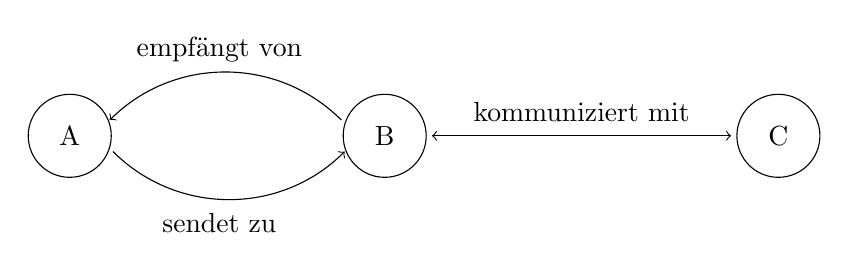
\begin{tikzpicture}
	\centering
	\draw (-4, 0) circle(15pt) node {A};
	\draw (0, 0) circle(15pt) node {B};
	\draw (5, 0) circle(15pt) node {C};
	\draw[->] (-0.55,0.2) arc (45:135:2.08);
	\draw[->] (-3.45,-0.2) arc (225:315:2.08);
	\draw[<->] (0.6,0) -- (4.4, 0);
	\draw  (-2.1, 1.1) node {empfängt von};
	\draw  (-2.1, -1.1) node {sendet zu};
	\draw  (2.5, 0.3) node {kommuniziert mit};
\end{tikzpicture}
\end{center}
\begin{enumerate}
\item Knotentyp A \textbf{sendet zu} einem Knoten vom Typ B.
\item Knotentyp B \textbf{empfängt von} einem Knoten von Typ A.
\item Knotentyp B \textbf{kommuniziert mit} einem Knoten vom Typ C.
\end{enumerate}
Die Idee unseres Ansatzes besteht nun darin passende Zeitpunkte zu definieren, zwischen denen entsprechende Beziehungen anhand von Netzwerkpaketen sichtbar sein müssen. Wir gehen davon aus, dass dies mit Hilfe der geforderten \textit{\Gls{Roundtriptime}} aus einem Pflichtenheft zuverlässig getan werden kann. Wir zeichnen daher den Netzwerkverkehr über ausreichend Zeit auf und klassifizieren unsere Knoten anhand der sichtbaren Beziehungen. Anomalien erkennt man daran, dass bei der Klassifikation mittels Inferenzmaschine Fehler auftreten, denn bei korrekter Modellierung ist damit ein Unterschied zum erwarteten Zustand aufgetreten und dadurch werden die definierten Regeln verletzt.

\section{\nohyphens{Mögliche Vorteile des Ansatzes}}
\label{chap:2:advantages}
Wie bereits bei der Diskussion zur Abbildung von Fehlern oder Soll-Zustand erwähnt, soll dieser Ansatz alle Fehler detektieren, die mit Hilfe von heuristischen Verfahren auf Netzwerkpaketen erkennbar sind. Ob dies mit unserer Realisierung bereits möglich ist, werden wir in Kapitel 5 evaluieren.\\
Aber das ist nicht der einzige mögliche Vorteil. Da \Glspl{Ontologie} außerhalb der Informatik bereits als Schnittstelle zum Wissensaustausch zwischen unterschiedlichen Quellen genutzt werden, bietet es sich an das hier ebenfalls zu tun. Denn eine geschriebene Ontologie bildet durch die definierten Beziehungen, Klassen und Individuen auch domänenspezifisches Wissen mit ab. Außerdem ist es möglich eine Vererbungshierarchie zwischen unterschiedlichen Ebenen von Ontologien aufzubauen und so bereits vorhandenes Wissen weiter zu verwenden oder zu abstrahieren, indem man auf Ontologien verweist. Dadurch kann dieses Modell gleichzeitig als Anomalieerkennung ,als Wissensdatenbank dienen und komplexe Klassen/Beziehungen können  in einfacher zu durchschauende zerlegt werden beziehungsweise daraus konkateniert werden.\\ Im Kontext der \acrlong{cps} kann es als Darstellung der Einzelnen Fertigungsschritte dienen und damit die gesamte Herstellungskette abbilden. Bisherige Ansätze sind auf maximal eine Firma beschränkt, da es als Risiko angesehen wird, solches Wissen durch Schnittstellen an Außenstehende zu geben. Auf der anderen Seite kann es aber das Aufspüren von defekten Chargen/Geräten deutlich vereinfachen, da man die Fertigungsdetails zurück verfolgen kann. \\
Ein weiterer Vorteil ist, dass es keine langwierigen Anlernphasen gibt. Wenn die Ontologie wohldefiniert ist, kann sie direkt ausgerollt und so als Erkennungssystem in der Inferenzmaschine genutzt werden. Außerdem ist es in unserem geplanten Szenario nicht nötig den Inhalt von Paketen zu inspizieren, wodurch Security- und Privacy-Interessen gewahrt bleiben.\\